\algnewcommand\algorithmicforeach{\textbf{for each}}
\algdef{S}[FOR]{ForEach}[1]{\algorithmicforeach\ #1\ \algorithmicdo}

\begin{figure}[t]
    \vspace{-15pt}
    \begin{minipage}[l]{0.55\textwidth}
    \begin{algorithm}[H]
    \begin{algorithmic}[1]
        \Require {
            student $\theta$,
            teacher $\Omega$,
            unlabeled LM data $\D_{LM}$,
            unlabeled transfer data $\D_{T}$,
            labeled data $\D_{L}$\newline
        }
        \State Initialize $\theta$ by pre-training an MLM$^+$ on $\D_{LM}$
        \ForEach {$x \in \D_T$}
            \State Get loss $L \gets -\sum_{y} P_\Omega(y | x) \log P_\theta(y | x)$
            \State Update student $\theta \gets \textsc{backprop}(L, \theta)$
        \EndFor
        \State Fine-tune $\theta$ on $\D_L$ \Comment{Optional step.}
        \State \Return $\theta$
    \end{algorithmic}
    \caption{}
    \end{algorithm}
    \end{minipage}
    %
    \hspace{10pt}
    %
    \begin{minipage}[l]{0.45\textwidth}
        \scalebox{0.8}{
        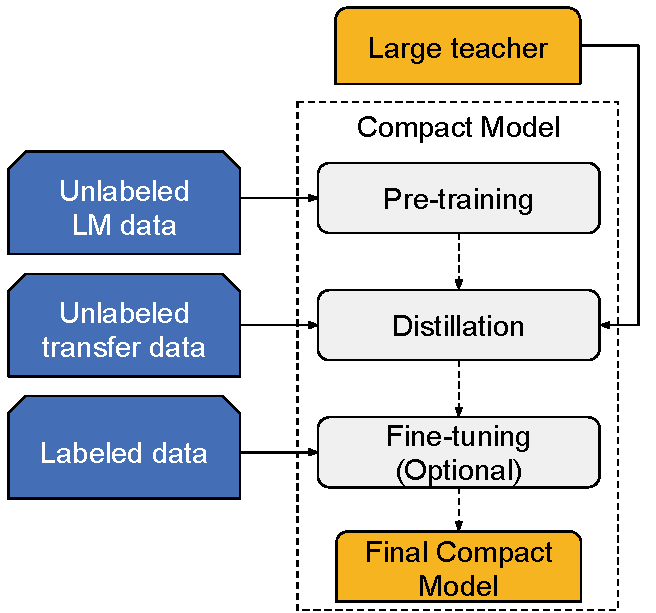
\includegraphics[width=\textwidth]{figures/recolored_our_recipe2.pdf}
        } % end scalebox
    \end{minipage}
    \caption{\recipename}
    \label{fig:pd}
\vspace{-10pt}
\end{figure}